\documentclass[svgnames,11pt]{beamer}
\input{/home/tof/Documents/Cozy/latex-include/preambule_commun.tex}
\input{/home/tof/Documents/Cozy/latex-include/preambule_beamer.tex}
%\usepackage{pgfpages} \setbeameroption{show notes on second screen=left}
\author[]{Christophe Viroulaud}
\title{Exercices ABR - correction}
\date{\framebox{\textbf{Algo 10}}}
%\logo{}
\institute{Terminale - NSI}

\begin{document}
\begin{frame}
    \titlepage
\end{frame}
\section{Exercice 1}
\begin{frame}
    \frametitle{Exercice 1}
    \begin{tabular}{ccc}
        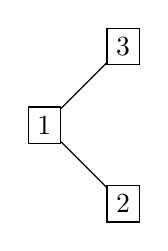
\begin{tikzpicture}
            \node[draw] (1) at (-1,-1) {1};
            \node[draw] (2) at (0,-2) {2};
            \node[draw] (3) at (0,0) {3};

            \draw (1) -- (2);
            \draw (3) -- (1);
        \end{tikzpicture}
         &
        \begin{tikzpicture}
            \node[draw] (1) at (-2,-2) {1};
            \node[draw] (2) at (-1,-1) {2};
            \node[draw] (3) at (0,0) {3};

            \draw (1) -- (2);
            \draw (3) -- (2);
        \end{tikzpicture}
         &
        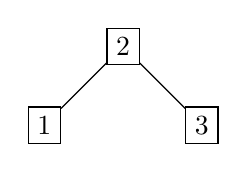
\begin{tikzpicture}
            \node[draw] (1) at (-1,-1) {1};
            \node[draw] (2) at (0,0) {2};
            \node[draw] (3) at (1,-1) {3};

            \draw (1) -- (2);
            \draw (3) -- (2);
        \end{tikzpicture}
        \\
        \begin{tikzpicture}
            \node[draw] (1) at (0,0) {1};
            \node[draw] (2) at (1,-1) {2};
            \node[draw] (3) at (2,-2) {3};

            \draw (1) -- (2);
            \draw (3) -- (2);
        \end{tikzpicture}
         &
        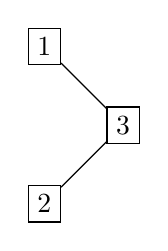
\begin{tikzpicture}
            \node[draw] (1) at (0,0) {1};
            \node[draw] (2) at (0,-2) {2};
            \node[draw] (3) at (1,-1) {3};

            \draw (1) -- (3);
            \draw (3) -- (2);
        \end{tikzpicture}
         & \\
    \end{tabular}



\end{frame}
\section{Exercice 2}
\begin{frame}
    \frametitle{Exercice 2}

    \begin{center}
        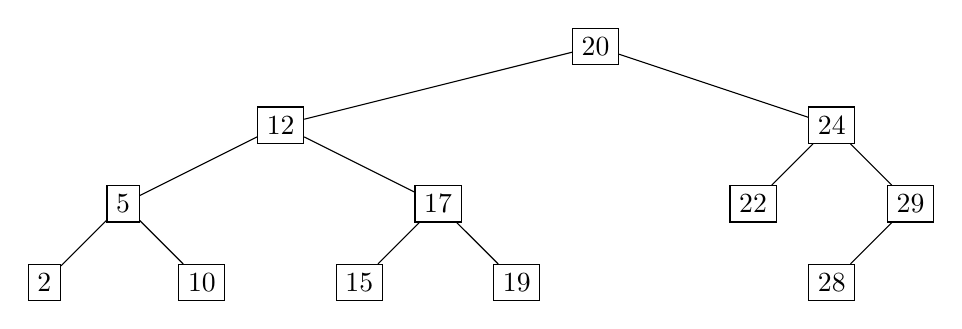
\begin{tikzpicture}
            \node[draw] (A) at (1,0) {20};
            \node[draw] (B) at (-3,-1) {12};
            \node[draw] (C) at (-5,-2) {5};
            \node[draw] (D) at (-1,-2) {17};
            \node[draw] (F) at (-4,-3) {10};
            \node[draw] (H) at (0,-3) {19};
            \node[draw] (I) at (4,-1) {24};
            \node[draw] (J) at (3,-2) {22};
            \node[draw] (K) at (-6,-3) {2};
            \node[draw] (L) at (-2,-3) {15};
            \node[draw] (M) at (5,-2) {29};
            \node[draw] (N) at (4,-3) {28};

            \draw (A) -- (B);
            \draw (C) -- (B);
            \draw (C) -- (F);
            \draw (D) -- (B);
            \draw (D) -- (H);
            \draw (A) -- (I);
            \draw (J) -- (I);
            \draw (K) -- (C);
            \draw (L) -- (D);
            \draw (M) -- (I);
            \draw (M) -- (N);
        \end{tikzpicture}
    \end{center}

    \begin{center}
        [2, 5, 10, 12, 15, 17, 19, 20, 22, 24, 28, 29]

    \end{center}
\end{frame}
\section{Exercice 3}
\begin{frame}[fragile]
    \frametitle{Exercice 3}

    \begin{center}
        \begin{lstlisting}[language=Python , basicstyle=\ttfamily\small, xleftmargin=0.5em, xrightmargin=0em]
class Noeud:
    def __init__(self, v: int):
        self.valeur = v
        self.gauche = None
        self.droit = None
\end{lstlisting}
    \end{center}

\end{frame}
\begin{frame}[fragile]

    \begin{center}
        \begin{lstlisting}[language=Python , basicstyle=\ttfamily\small, xleftmargin=0.5em, xrightmargin=0em]
def inserer(self, v: int) -> None:
    if v < self.valeur:  # gauche
        if self.gauche is None:  # feuille
            self.gauche = Noeud(v)
        else:  # descente récursive
            self.gauche.inserer(v)
    else:  # droite
        if self.droit is None:  # feuille
            self.droit = Noeud(v)
        else:  # descente récursive
            self.droit.inserer(v)
\end{lstlisting}
    \end{center}

\end{frame}
\begin{frame}[fragile]

    \begin{center}
        \begin{lstlisting}[language=Python , basicstyle=\ttfamily\small, xleftmargin=0.5em, xrightmargin=0em]
arbre = Noeud(13)
arbre.inserer(29)
arbre.inserer(2)
arbre.inserer(49)
arbre.inserer(8)
arbre.inserer(12)
arbre.inserer(16)
arbre.inserer(30)
arbre.inserer(27)
arbre.inserer(10)
arbre.inserer(9)
\end{lstlisting}
    \end{center}

\end{frame}
\begin{frame}[fragile]

\begin{center}
\begin{lstlisting}[language=Python , basicstyle=\ttfamily\small, xleftmargin=0.5em, xrightmargin=0em]
def rechercher(self, v: int) -> None:
    if v == self.valeur: # trouvé
        return True
    elif v < self.valeur:  # gauche
        if self.gauche is None:  # feuille
            return False
        else:  # descente récursive
            return self.gauche.rechercher(v)
    else:  # droite
        if self.droit is None:  # feuille
            return False
        else:  # descente récursive
            return self.droit.rechercher(v)
\end{lstlisting}
\end{center}

\end{frame}
\begin{frame}[fragile]

\begin{center}
\begin{lstlisting}[language=Python , basicstyle=\ttfamily\small, xleftmargin=0.5em, xrightmargin=0em]
print(arbre.rechercher(16))  # True
print(arbre.rechercher(17))  # False
\end{lstlisting}
\end{center}
    
    \end{frame}
\begin{frame}[fragile]

\begin{center}
\begin{lstlisting}[language=Python , basicstyle=\ttfamily\small, xleftmargin=0.5em, xrightmargin=0em]
def minimum(self) -> int:
    n = self # instance en cours
    while n.gauche is not None:
        n = n.gauche
    return n.valeur


def minimum_rec(self) -> int:
    if self.gauche is None:
        return self.valeur
    else:
        return self.gauche.minimum_rec()
\end{lstlisting}
\end{center}

\end{frame}
\begin{frame}[fragile]

\begin{center}
\begin{lstlisting}[language=Python , basicstyle=\ttfamily\small, xleftmargin=0.5em, xrightmargin=-2.5em]
def infixe(self, parcours: list) -> None:
    if self.gauche is not None:
        self.gauche.infixe(parcours)
    parcours.append(self.valeur)
    if self.droit is not None:
        self.droit.infixe(parcours)
\end{lstlisting}
\end{center}
    
    \end{frame}
\section{Exercice 4}
\begin{frame}[fragile]
    \frametitle{Exercice 4}

\begin{center}
\begin{lstlisting}[language=Python , basicstyle=\ttfamily\small, xleftmargin=.3em, xrightmargin=-3em]
def taille(a: dict, s: str) -> int:
    if a[s][0] == '' and a[s][1] == '':  # pas de fils
        return 1
    elif a[s][0] == '':  # pas de fils gauche
        return 1 + taille(a, a[s][1])
    elif a[s][1] == '':  # pas de fils droit
        return 1 + taille(a, a[s][0])
    else:  # deux fils
        return 1 + taille(a, a[s][1]) + taille(a, a[s][0])
\end{lstlisting}
\end{center}    

\end{frame}
\end{document}